\chapter{Stochastische Modelle in der Robotik}\pdfcomment{Zusammenhangsloser Quatsch}
Jede elaborierte Methoden erfordert einen Rahmen, in dem sie erarbeitet, formuliert und optimiert werden kann. In technischen Aufgabenstellung erfüllt die Mathematik diese Forderungen, weshalb die Gegebenheiten und Probleme des hiesigen Anwendungsfall zunächst in einem mathematischen Kontext dargestellt werden. Denn nur von dieser Basis ausgehend, besteht die Aussicht auf eine elegante und ansprechende Lösung.

Wie alle Probleme der Robotik, kann auch die autonome Navigation im entferntesten Sinne als Interaktion eines Roboters mit seiner Umwelt aufgefasst werden. Anhand von gesammelten Informationen muss das System eine Entscheidung über seine zukünftigen Aktionen treffen, wobei ein entferntes Ziel ohne ungewollte Kollisionen angesteuert werden soll. Für diese Aufgaben spielen drei Größen eine fundamentale Rolle. Zunächst muss die Position des Roboters beachtet werden, welche in dem Positionsvektor $\mVec{x}(t) \equiv \mVec{x}_t$ erfasst wird. Mithilfe von Sensoren sammelt der Roboter Informationen über seine Umgebung, die in dem Messvektor $\mVec{z}_t$ zusammengefasst werden. Anhand der Mess- und Positionsvektoren wird über die nächste Aktion des Roboters entschieden, die in dem Steuervektor $\mVec{u}_t$ ausgedrückt wird. Die exakte Form der Positions-, Mess- und Steuervektoren hängt von dem gegebenen Anwendungsfall und gewählten Modellformen ab, die im Folgenden näher erläutert werden.

In anderen Fachgebieten, die sich mit der Planung von Steuersignalen bzw. -sequenzen beschäftigen - wie z.B. die Regelungstechnik -, haben sich modellbasierte Methoden bewährt. Zunächst wird auf Basis von physikalischen Gegebenheiten der Zusammenhang zwischen Steuer-, Zustands- und Messvektor hergeleitet, der anschließend genutzt wird, um eine Regelstrategie zu formulieren. Der resultierende Algorithmus berechnet die Stellgröße $\mVec{u}_t$, wofür die aktuellen Mess- und Zustandsvektoren herangezogen werden. Insofern liegt es nahe modellbasierte Ansätze auch bei Problemen der Robotik zu verfolgen. Allerdings kommt dort die ungemeine Komplexität der Problemstellung zu tragen, die sich recht leicht am Beispiel der Navigation illustrieren lässt: Als erstes muss ein Modell für den Einfluss des Stellvektors $\mVec{u}_t$ auf den Positionsvektor $\mVec{x}_t$ erstellt werden. Bei mobilen Roboterplattformen handelt es sich um mechanische Systeme mit mehreren Freiheitsgraden, womit die analytische Modellbildung zwar möglich, jedoch mit einem beachtlichen Aufwand verbunden ist. Spätestens bei der Modelierung der Sensoren werden die Grenzen des Möglichen erreicht: Soll beispielsweise die Position des Roboters mithilfe von Stereokameras erfasst werden kann praktisch kaum ein exaktes, deterministisches Modell für diesen Vorgang erfasst werden, da er von zu vielen unbekannten Einflussfaktoren betroffen ist. Zuletzt kann die Pfadplanung per Definition nicht anhand eines deterministischen Modell erfolgen, da der Roboter dynamischen Hindernissen ausweichen soll, deren Form und Bewegung in der Aufgabenstellung nicht näher spezifiziert werden.

Aus diesen Gründen haben sich in der Robotik stochastische Modellformen etabliert, wobei recht simple Ausgangsmodelle verwendet werden, die um Zufallsvariablen ergänzt werden, um die Ungenauigkeiten und Ungewissheiten des Modells zu repräsentieren. Das Ziel besteht nicht mehr darin, konkrete Aussagen über den Verlauf von Zustandsgrößen zu treffen, wie dies z.B. bei einer Zustandsraumdarstellung der Form
\begin{equation}
\mVec{x}(n+1) = \mat{{A}}\cdot \mVec{x}(n) + \mat{B}\cdot \mVec{\mathbf{u}}(n)
\end{equation}
erfolgt. Vielmehr soll mithilfe des Modells eine bedingte Wahrscheinlichkeit
\begin{equation}
\condP{\mVec{x}(n+1)}{\mVec{x}(n), \mVec{u}(n)}
\end{equation}
berechnet werden. Im Anschluss können die Methoden der Wahrscheinlichkeitstheorie genutzt werden, um Filter- und Planungsalgorithmen zu entwerfen.\pdfcomment{Wiederholung der um.. Konstruktion} Um einen ersten Eindruck für diese Modellformen zu erhalten, werden im Anschluss rudimentäre Ansätze für ein Bewegungs- und Sensormodell vorgestellt.


\newpage
\section{Geschwindigkeitsbasiertes Bewegungsmodell } \footnote{Das Bewegungsmodell und dessen Herleitung stammen aus \cite[S. 121 ff]{ProbRob}} 
Als erstes Beispiel wird ein stochastisches Modell für die Roboterbewegung entworfen, wobei anhand des vergangenen Positionsvektor $\mVec{x}_{t-1}$ und des aktuellen Steuervektors $\mVec{u}_t$ die Wahrscheinlichkeitsverteilung des aktuellen Positionsvektors $\mVec{x}_t$
\begin{equation}
\condP{\mVec{x}_t}{\mVec{u}_t, \mVec{x}_{t-1}}
\end{equation}
bestimmt werden soll. In diesem Fall wird lediglich eine planare Bewegung betrachtet, das heißt der Roboter bewegt sich in der xy-Ebene. Der Positionsvektor setzt sich somit aus den drei Größen
\begin{equation}
\mVec{x} = \begin{pmatrix}
x \\ y \\ \theta
\end{pmatrix}
\end{equation}
zusammen, welche die x-/y-Position und Ausrichtung des Roboters wiedergeben. $\theta$ gibt dabei den Winkel zwischen der x-Koordinatenachse und der Blickrichtung des Roboters an.
Der Steuervektor $\mVec{u}$ gibt die aktuelle Translations- und Rotationsgeschwindigkeit
\begin{equation}
\mVec{u} = \begin{pmatrix}
v \\ \omega
\end{pmatrix}
\end{equation}
des Roboters an, wobei angenommen wird, dass die beiden Geschwindigkeiten zwischen zwei Abtastpunkten $t$ und $t+1$ konstant sind. $v$ beschreibt die Translationsgeschwindigkeit in Blickrichtung, während $\omega$ die Änderung des Blickwinkels $\theta$ wiedergibt.
Unter der Annahme dass die Geschwindigkeiten $\mVec{u}$ in dem Intervall $]t-1, t]$ zwischen zwei Abtastpunkten konstant bleibt, kann die Bewegung als Rotation um einen konstanten Momentanpol $\mVec{c} = \begin{pmatrix} x_c & y_c \end{pmatrix}^T$ betrachtet werden.
\begin{figure}[!ht]
\centering
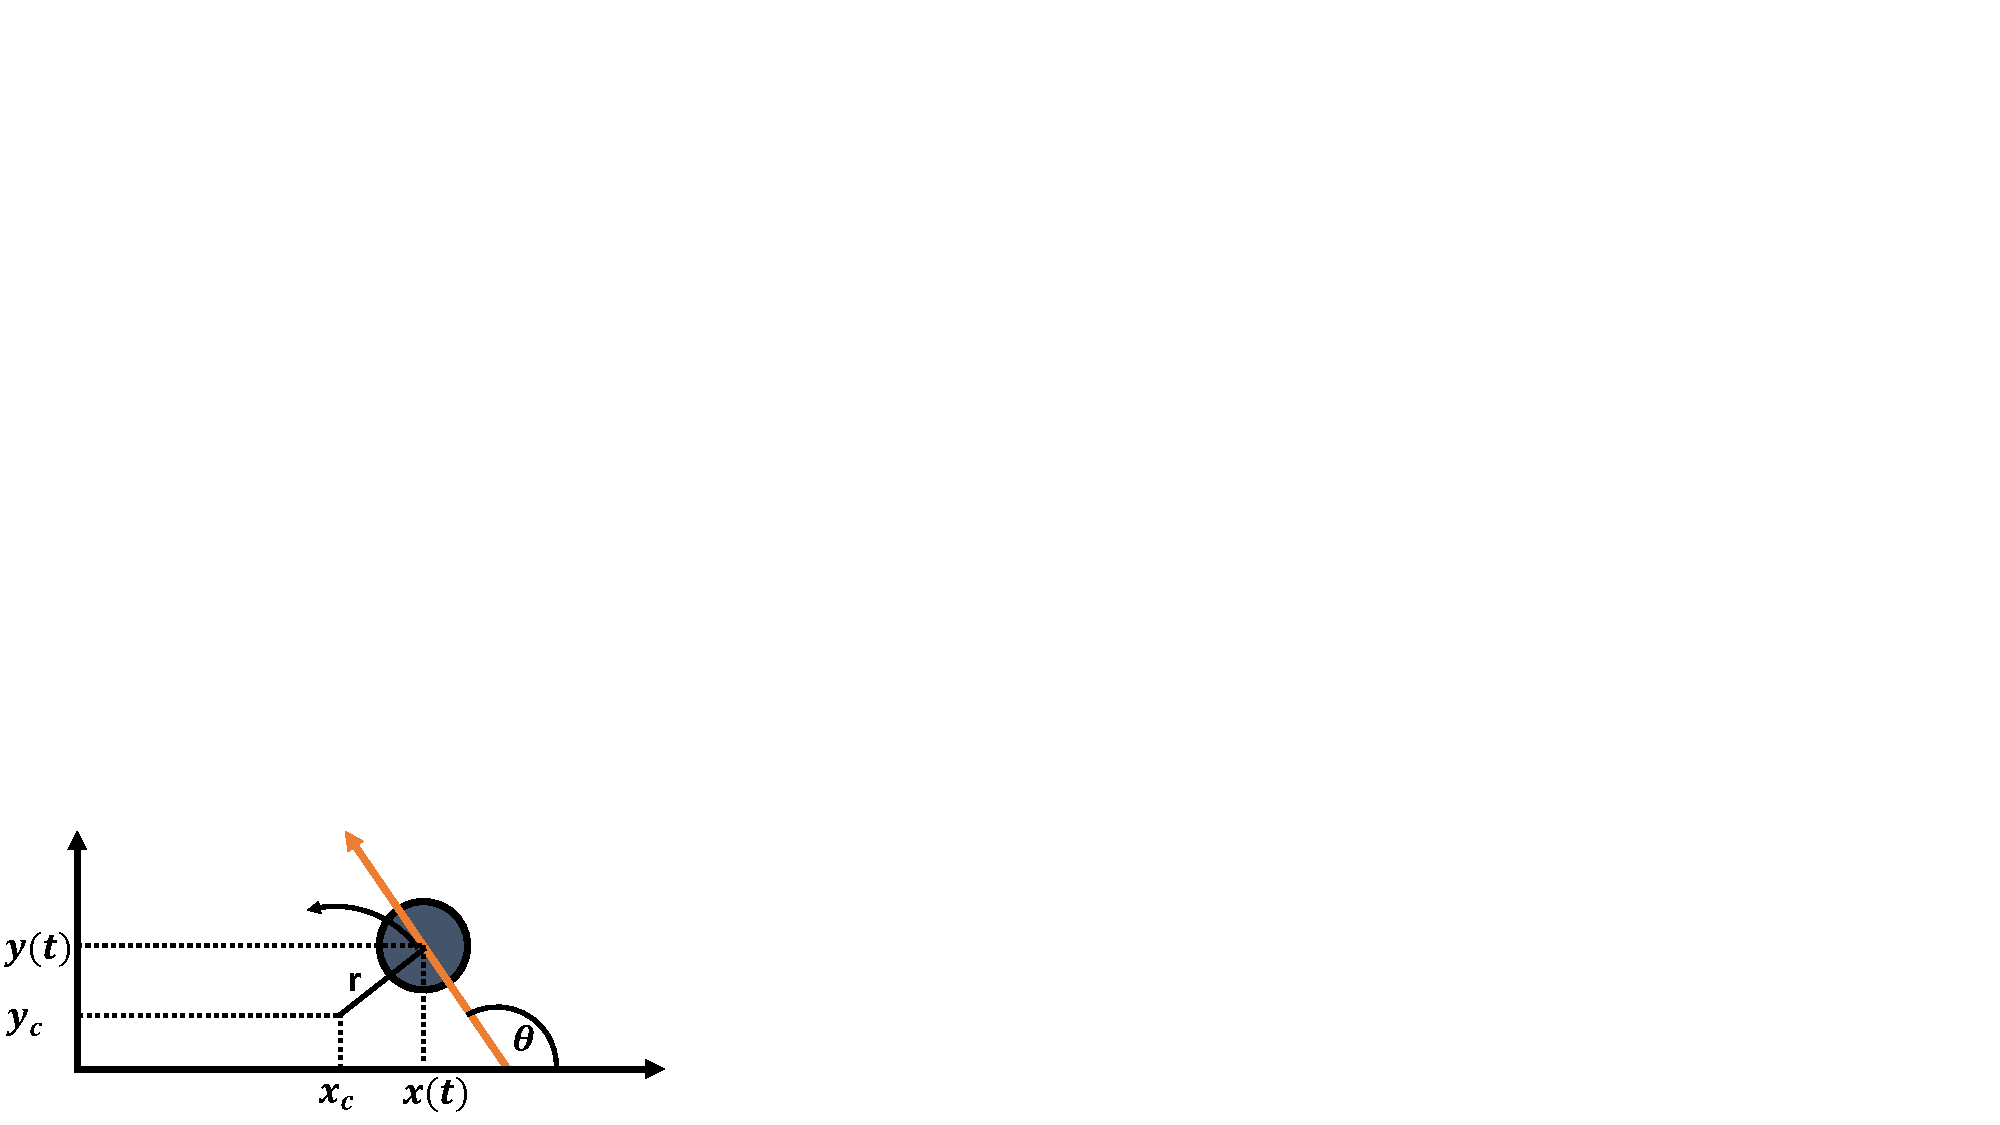
\includegraphics[width=0.6\linewidth, trim={0cm 0cm 24cm 14cm}, clip]{img/Bild_Kinematik_1}
\caption{Darstellung des Momentanpols am Zeitpunkt $t$ \cite[S. 126]{ProbRob}}
\end{figure}

Für den Radius gilt
\begin{equation}
r = \left\vert \frac{v}{\omega}\right\vert\,,
\end{equation}
wobei zu beachten ist, dass der Radius für eine Winkelgeschwindigkeit $\omega=0$ gegen unendlich konvergiert, was wiederum einer reinen Translation entspricht. Aus dem Positionsvektors des Roboters $\mVec{x}_t$ an dem Zeitpunkt $t$ kann der Momentanpol für die folgende Abtastperiode berechnet werden:
\begin{equation}
\label{eq_kinematic_1}
\begin{pmatrix}
x_c \\ y_c
\end{pmatrix} = \begin{pmatrix}
x(t) - \frac{v}{\omega}\cdot \mySin{\theta} \\ y(t) + \frac{v}{\omega}\cdot \myCos{\theta}
\end{pmatrix} \hspace{15pt}\leftrightarrow\hspace{15pt} 
\begin{pmatrix}
x(t) \\ y(t)
\end{pmatrix} = \begin{pmatrix}
x_c + \frac{v}{w}\cdot \mySin{\theta} \\ y_c - \frac{v}{w}\cdot \myCos{\theta}
\end{pmatrix}\,.
\end{equation}
Im nächsten Schritt wird die Bewegung über eine Abtastperiode $\Delta t$ betrachtet, wodurch der Roboter um die Winkeldifferenz $\Delta t\cdot \omega$ auf dem Kreisbogen wandert. Nach \ref{eq_kinematic_1} folgt für den Positionsvektor am Zeitpunkt $t+\Delta t$
\begin{equation}
\label{eq_kinematic_2}
\begin{split}
\begin{pmatrix}
x(t+\Delta t) \\ y(t+\Delta t) \\ \theta(t+\Delta t
\end{pmatrix} &= \begin{pmatrix}
x_c + \frac{v}{w}\cdot \mySin{\theta(t)+\omega\cdot \Delta t} \\ y_c - \frac{v}{w}\cdot \myCos{\theta(t)+\omega \cdot \Delta t} \\ \theta(t) + \omega\cdot \Delta t
\end{pmatrix}\\
& = \begin{pmatrix}
x(t) \\ y(t) \\ \theta(t)
\end{pmatrix} + \begin{pmatrix}
-\frac{v}{\omega}\cdot\mySin{\theta(t)} + \frac{v}{\omega}\cdot \mySin{\theta(t)+\omega \cdot \Delta t} \\
\frac{v}{\omega}\cdot \myCos{\theta(t)} - \frac{v}{w}\cdot \myCos{\theta(t)+\omega \cdot \Delta t}\\
\omega\cdot \Delta t
\end{pmatrix}\,.
\end{split}
\end{equation}
Bisher wurden lediglich deterministische Bewegungen betrachtet. Um nun mögliche Fehler des Steuervektors $\mVec{u}$ zu beachten, werden die störbehafteten Geschwindigkeiten
\begin{equation}
\mVec{u} = \begin{pmatrix}
\hat{v} \\ \hat{\omega}
\end{pmatrix} = \begin{pmatrix}
v + v\idx{err} \\ \omega + \omega\idx{err}
\end{pmatrix}
\end{equation}
eingeführt. Die Zufallsvariablen $v\idx{err}$ und $\omega\idx{err}$ dienen der Fehlermodellierung und ihre Wahrscheinlichkeitsverteilungen $\varepsilon_v$ und $\varepsilon_\omega$ werden dem Anwendungsfall nach angepasst. Einsetzen des stochastischen Steuervektors $\mVec{u}$ liefert
\begin{equation}
\begin{pmatrix}
x(t+\Delta t) \\ y(t+\Delta t) \\ \theta(t+\Delta t
\end{pmatrix} 
=
\begin{pmatrix}
x(t) \\ y(t) \\ \theta(t)
\end{pmatrix} + \begin{pmatrix}
-\frac{\hat{v}}{\hat{\omega}}\cdot\mySin{\theta(t)} + \frac{\hat{v}}{\hat{\omega}}\cdot \mySin{\theta(t)+\hat{\omega} \cdot \Delta t} \\
\frac{\hat{v}}{\hat{\omega}}\cdot \myCos{\theta(t)} - \frac{\hat{v}}{w}\cdot \myCos{\theta(t)+\hat{\omega} \cdot \Delta t}\\
\hat{\omega}\cdot \Delta t
\end{pmatrix}\,.
\end{equation}
In diesem Modell wurden lediglich zwei Zufallsvariablen eingeführt, um die Störung von drei Positionsvariablen zu modellieren. Aus diesem Grund entsteht eine ungewollte stochastische Abhängigkeit zwischen den Elementen des Positionsvektors $\mVec{x}(t+\Delta t)$. Dieses Problem wird behoben, indem eine dritte Zufallsvariable
\begin{equation}
\gamma\idx{err} \equiv \hat{\gamma}
\end{equation}
eingeführt wird, die zu einer zusätzlichen Störung der Orientierung $\theta(t+\Delta t)$ in Form von
\begin{equation}
\label{eq_kinematic_3}
\begin{pmatrix}
x(t+\Delta t) \\ y(t+\Delta t) \\ \theta(t+\Delta t
\end{pmatrix} 
=
\begin{pmatrix}
x(t) \\ y(t) \\ \theta(t)
\end{pmatrix} + \begin{pmatrix}
-\frac{\hat{v}}{\hat{\omega}}\cdot\mySin{\theta(t)} + \frac{\hat{v}}{\hat{\omega}}\cdot \mySin{\theta(t)+\hat{\omega} \cdot \Delta t} \\
\frac{\hat{v}}{\hat{\omega}}\cdot \myCos{\theta(t)} - \frac{\hat{v}}{w}\cdot \myCos{\theta(t)+\hat{\omega} \cdot \Delta t}\\
\hat{\omega}\cdot \Delta t + \hat{\gamma}\cdot \Delta t
\end{pmatrix}
\end{equation}
führt. Die Aufgabe besteht jetzt darin, ein Bewegungsmodell in Form der bedingten Wahrscheinlichkeit
\begin{equation}
\condP{\mVec{x}_t]}{\mVec{u}_t, \mVec{x}_{t-1}}
\end{equation}
zu formulieren. Das heißt es soll eine Funktion aufgestellt werden, die berechnet wie wahrscheinlich der Zustand $\mVec{x}_t$ auf den Zustand $\mVec{x}_{t-1}$ und die Aktion $\mVec{u}_t$ folgt. Dafür wird nach Gleichung (\ref{eq_kinematic_3}) die Werte der stochastisch unabhängigen Zufallsvariablen $v\idx{err}$, $\omega\idx{err}$ und $\gamma\idx{err}$ berechnet. Die gesuchte Wahrscheinlichkeit ergibt sich dann aus deren gemeinsamer Verteilung
\begin{equation}
p(\mVec{x}_t, \mVec{u}_t, \mVec{x}_{t-1}) = \condP{\mVec{x}_t}{\mVec{u}_t, \mVec{x}_{t-1}} = \varepsilon_v(v\idx{err})\cdot \varepsilon_\omega(\omega\idx{err})\cdot \varepsilon_\gamma(\gamma\idx{err})\,.
\end{equation}
Da die direkte Umformung von Gleichung (\ref{eq_kinematic_1}) zur expliziten Darstellung der gesuchten Fehlergrößen zu einem unhandlichen Ergebnis führt, wird eine indirekte Berechnung über den Momentanpol gewählt. Im ersten Schritt werden die Koordinaten des Momentanpols $\mVec{c}$ berechnet, wofür sich nach \cite[S. 130]{ProbRob} \footnote{Schreibweise für $\mVec{x}_t = \begin{pmatrix}
x & y &\theta
\end{pmatrix}^T$, $\mVec{x}_{t+\Delta t} = \begin{pmatrix}
\tilde{x} & \tilde{y} &\tilde{\theta}
\end{pmatrix}^T$}
\begin{equation}
\begin{pmatrix}
x_c \\ y_c
\end{pmatrix} = \begin{pmatrix}
\frac{x+\tilde{x}}{2} + \mu (y-\tilde{y})\\ \frac{y+\tilde{y}}{2}+\mu(\tilde{x}-x)
\end{pmatrix} \hspace{1.5cm}
\mu = \frac{1}{2}\frac{(x-\tilde{x})\myCos{\theta} + (y-\tilde{y})\mySin{\theta}}{(y-\tilde{y})\myCos{\theta}-(x-\tilde{x})\mySin{\theta}}
\end{equation}
ergibt. Woraus sich sowohl der Rotationsradius
\begin{equation}
r\idx{c} = \sqrt{(x-x_c)^2+(y-y_c)^2}
\end{equation}
als auch der auf der Kreisbahn zurückgelegte Winkel 
\begin{equation}
\Delta \theta = \myAtan{\frac{\tilde{y}-y_c}{\tilde{x}-x_c}}-\myAtan{\frac{y-y_c}{x-x_c}}
\end{equation}
berechnen lassen. Mithilfe der der Winkeldifferenz lässt sich wiederum auf die zurückgelegte Strecke
\begin{equation}
\Delta s = r\idx{c}\cdot \Delta \theta
\end{equation}
schließend, welche zusammen auf den gestörten Stellvektor
\begin{equation}
\mVec{\hat{u}} = \begin{pmatrix}
\hat{v}\\ \hat{\omega}
\end{pmatrix} = \frac{1}{\Delta t}\cdot \begin{pmatrix}
\Delta s\\ \Delta \theta
\end{pmatrix}
\end{equation}
führen. Zuletzt fehlt der Orientierungsfehler $\hat{\gamma}$, der sich mithilfe von Gleichung (\ref{eq_kinematic_3}) erschließen lässt.
\begin{equation}
\tilde{\theta}-\theta = \hat{\omega}\cdot \Delta t + \hat{\gamma}\cdot \Delta t
\Leftrightarrow
\hat{\gamma} = \frac{\tilde{\theta}-\theta}{\Delta t} - \hat{\omega}\,.
\end{equation}

\newpage
\section{Messmodell}
Als weiteres Beispiel wird ein stochastisches Messmodell vorgestellt, das später bei der Lokalisierung wiederverwendet wird. Das Ziel des Messmodells ist es den Zusammenhang zwischen einem Zustandsvektor $\mVec{x}\idx{t}$ und einem Messvektor $\mVec{z}\idx{t}$ in Form der bedingten Wahrscheinlichkeit
\begin{equation}
\condP{\mVec{z}\idx{t}}{\mVec{x}\idx{t}}
\end{equation}
herzustellen. Die Verteilung sagt aus, mit welcher Wahrscheinlichkeit ein Messvektor $\mVec{z}\idx{t}$ von einer vorgegebenen Position $\mVec{x}\idx{t}$ aus erzielt wird. Das Messmodell dient als Paradebeispiel dafür, wie heuristische Argumente in stochastische Modelle einfließen können. Unabhängig von dem exakten Sensor wird angenommen, dass es sich um ein auf Messstrahlen basiertes Messprinzip handelt. Das heißt der Messvektor $\mVec{z}\idx{t}$ setzt sich aus mehreren Messwerten $z^k\idx{t}$ zusammen, die jeweils die auf einem Strahl gemessene Distanz wiedergeben. 

Als erste Störgröße wird ein gewöhnliches Messrauschen eingeführt, das als normal verteilt angenommen wird. Der Mittelwert der Verteilung sie die tatsächliche Distanz auf dem Messstrahl, die mit $z^{k*}\idx{t}$ denotiert wird. Als zweiter Parameter muss die Varianz $\sigma\idx{hit}$ festgelegt werden, die angibt wie stark der Messwert von dem Rauschen beeinflusst wird. Somit ergibt sich als Modell für das Sensorrauschen
\begin{equation}
p\idx{hit}\left( z^{k}\idx{t} \mCond \mVec{x}\idx{t} \right) = \left\{ \begin{array}{cl}
\eta \cdot \mathcal{N}(z^k\idx{t}, z^{k*}\idx{t}, \sigma^2\idx{hit}) & \hspace{5mm}\forall z^k\idx{t} \in \left[0, z\idx{max}\right] \\
0 & \hspace{5mm} \forall z^k\idx{t} \notin \left[0, z\idx{max}\right]
\end{array}\right. \,.
\end{equation}
Die Messwerte werden außerdem von unerwarteten Objekten beeinflusst. Angenommen es liegt eine Karte der Umgebung vor und es bewegt sich ein Mensch innerhalb des Raumes. Wenn der Mensch nun die Messstrahlen unterbricht tritt ein geringerer Messwert als anhand der Karte erwartet ein. Im Allgemeinen gilt, dass im Falle von Störungen durch unerwartete Objekte die Messwerte lediglich kleiner, aber niemals größer werden. Des Weiteren nimmt die Wahrscheinlichkeit, dass ein Messwert von einem Objekt beeinflusst wird mit zunehmendem Messdistanz ab. Für das Modell wird eine exponentiell abfallende Verteilung
\begin{equation}
\renewcommand*{\arraystretch}{1.3}
p\idx{short}\left( z^k\idx{t} \mCond \mVec{x}\idx{t} \right) = \left\{ \begin{array}{cl}
\eta \cdot \lambda\idx{short}\cdot e^{-\lambda\idx{short}\cdot z^{k}\idx{t}} & \hspace{5mm} \forall z^{k}\idx{t} \in \left[0, z^{k*}\idx{t}\right] \\
0 & \hspace{5mm} \forall z^{k}\idx{t} \notin \left[0, z^{k*}\idx{t}\right]
\end{array}\right. 
\end{equation}
gewählt, wobei $\lambda\idx{short}$ als wählbarer Parameter die Häufigkeit der Störungen widerspiegelt.

Als dritte Ursache für Messfehler wird das sporadische Versagen des Sensors herangezogen. Derartige Phänomene können bei Laserscannern auftreten, wenn beispielsweise schwarze Oberflächen die Strahlen vollständig absorbieren. Ähnliche Probleme werden bei Sonarsensoren durch Interferenz oder schallabsorbierende Medien hervorgerufen. Unabhängig von dem Messprinzip des Sensors werden in all den beschriebenen Fällen - fälschlicherweise - maximale Distanzen gemessen, wodurch die Verteilung
\begin{equation}
p\idx{max}\left(z^k\idx{t} \mCond \mVec{x}\idx{t}\right) = \left\{ \begin{array}{cl}
1 & \hspace{5mm} \forall z = z\idx{max} \\
0 & \hspace{5mm} \forall z  \neq z\idx{max}
\end{array}\right.
\end{equation}
motiviert wird. {\color{red} Die Aussage von dieser Verteilung ist ein bisschen Banane, wenn wenn der Messwert den maximal Möglichen anzeigt, ist die dass 100 Prozent der Fall, ansonsten nicht? Oder ist es so zu verstehen, dass ein maximaler Messwert zu 100 Prozent den Fall von Messfehler bedeutet? Dann müsste ich die Interpretation der anderen Verteilungen nochmal überdenken}

Als letzter und absurdester Fall werden rein zufällig falsche Phänomene betrachtet. Als Argument dient die Beobachtung, dass es unerklärliche Messwerte gibt, die - zu Gunsten der Simplizität - durch eine Gleichverteilung der Form
\begin{equation}
\renewcommand*{\arraystretch}{1.3}
p\idx{rand}\left( z^k\idx{t} \mCond \mVec{x}\idx{t}\right) = \left\{ \begin{array}{cl}
\frac{1}{z\idx{max}} & \hspace{5mm} \forall z^k\idx{t} \in \left[0, z\idx{max}\right] 
\\
0 & \hspace{5mm} \forall z^k\idx{t} \notin \left[0, z\idx{max}\right]
\end{array} \right.
\end{equation}
repräsentiert werden. Es liegt schließlich nahe das komplexeste aller Probleme durch die simpelste aller Darstellung zu beschreiben. An diesem Beispiel wird deutlich, dass heuristische Einflüsse in stochastischen Modellen auch mit variierendem Elan verteidigt werden.

Die gesuchte Wahrscheinlichkeit $\condP{z^k\idx{t}}{\mVec{x}\idx{t}}$ wird aus Summe der vier Verteilung berechnet, wobei diese mit den Faktoren $z\idx{hit}$, $z\idx{short}$, $z\idx{max}$ und $z\idx{rand}$ gewichtet werden. Die Gewichtung erlauben es dem Anwender, die Heuristiken nach ihrer Glaubhaftigkeit zu bewerten.
\begin{equation}
\condP{z^k\idx{t}}{\mVec{x}\idx{t}} = \begin{bmatrix} z\idx{hit} & z\idx{short} & z\idx{max} z\idx{rand} \end{bmatrix} \cdot \begin{bmatrix}
p\idx{hit}\left( z^{k}\idx{t} \mCond \mVec{x}\idx{t} \right) \\
p\idx{short}\left( z^k\idx{t} \mCond \mVec{x}\idx{t} \right) \\
p\idx{max}\left(z^k\idx{t} \mCond \mVec{x}\idx{t}\right) \\
p\idx{rand}\left( z^k\idx{t} \mCond \mVec{x}\idx{t}\right)
\end{bmatrix}\,.
\end{equation}
\newpage
\section{Kontinuierliches Bayes Filter}
In der Robotik werden stochastische Filter genutzt, um anhand von gegebenen Information wie Mess- und Stellgrößen eine Schätzung über unbekannte Zustände des Systems zu treffen. Die Grundlage für derartige Methoden stellt das Bayes-Filter für kontinuierlich verteilte Zustände dar. Als Beispiel für die Herleitung und Illustration des Filters wird die Lokalisierungsaufgabe herangezogen, bei welcher die aktuelle Position $\mVec{x}\idx{t}$ des Roboters ermittelt werden soll. Die Schätzung stützt sich dabei auf die bisher gesammelten Messwerte $\mVec{z}\idx{1:t}$ und Stellgrößen $\mVec{u}\idx{1:t}$. Insofern kann die Lokalisierungsaufgabe als die Bestimmung der bedingten Wahrscheinlichkeit
\begin{equation}
\condP{\mVec{x}\idx{t}}{\mVec{z}\idx{1:t},\mVec{u}\idx{1:t}}
\end{equation}
reformuliert werden, die im Folgenden auch mittels der Definition
\begin{equation}
\bel{\mVec{x}\idx{t}} \equiv \condP{\mVec{x}\idx{t}}{\mVec{z}\idx{1:t},\mVec{u}\idx{1:t}}
\end{equation}
abgekürzt wird. Im Falle, dass der aktuelle Messwert $\mVec{z}\idx{t}$ bei der Verteilung nicht beachtet wird, gilt
\begin{equation}
\pbel{\mVec{x}\idx{t}} \equiv \condP{\mVec{x}\idx{t}}{\mVec{z}\idx{1:t-1},\mVec{u}\idx{1:t}}\,.
\end{equation}
Für die Bestimmung der Filtergleichungen wird auf Bayes Theorem zurückgegriffen:
\begin{equation}
\begin{split}
\bel{\mVec{x}\idx{t}} &= \condP{\mVec{x}\idx{t}}{\mVec{z}\idx{t},\mVec{z}\idx{1:t-1},\mVec{u}\idx{1:t}} = \frac{ \condP{\mVec{z}\idx{t}}{\mVec{x}\idx{t},\mVec{z}\idx{1:t-1},\mVec{u}\idx{1:t}}\cdot \condP{\mVec{x}\idx{t}}{\mVec{z}\idx{1:t-1},\mVec{u}\idx{1:t}}}{\condP{\mVec{z}\idx{t}}{\mVec{z}\idx{1:t-1}, \mVec{u}\idx{1:t}}}
\\
&= \mu \cdot \condP{\mVec{z}\idx{t}}{\mVec{x}\idx{t},\mVec{z}\idx{1:t-1},\mVec{u}\idx{1:t}}\cdot \condP{\mVec{x}\idx{t}}{\mVec{z}\idx{1:t-1},\mVec{u}\idx{1:t}}\,.
\end{split}
\end{equation}
Der Einfluss der bedingte Wahrscheinlichkeit $\condP{\mVec{z}\idx{t}}{\mVec{z}\idx{1:t-1}, \mVec{u}\idx{1:t}}$ wird dabei durch den Faktor $\mu$ ersetzt, der für die Normalisierung reserviert wird, um sicherzustellen, dass es sich bei $\pbel{\mVec{x}\idx{t}}$ um eine legitime Wahrscheinlichkeitsverteilung handelt. Eine weitere Vereinfachung basiert auf der Annahme, dass $\mVec{x}\idx{t}$ einen so genannten vollständigen Zustand darstellt, das heißt $\mVec{x}\idx{t}$ beinhaltet bereits alle vergangen Information. Aus diesem Grund verändern zusätzliche Informationen aus vergangen Mess- und Stellgrößen eine mit $\mVec{x}\idx{t}$ bedingte Wahrscheinlichkeit nicht, woraus 
\begin{equation}
\condP{\mVec{z}\idx{t}}{\mVec{x}\idx{t},\mVec{z}\idx{1:t-1},\mVec{u}\idx{1:t}} = \condP{\mVec{z}\idx{t}}{\mVec{x}\idx{t}}
\end{equation}
resultiert. Wird dieses Ergebnis in die ursprüngliche Gleichung eingesetzt, ergibt sich
\begin{equation}
\label{eq_contbayes2}
\begin{split}
\bel{\mVec{x}\idx{t}} &= \mu \cdot \condP{\mVec{z}\idx{t}}{\mVec{x}\idx{t}}\cdot \condP{\mVec{x}\idx{t}}{\mVec{z}\idx{1:t-1},\mVec{u}\idx{1:t}} 
\\
&= \mu \cdot \condP{\mVec{z}\idx{t}}{\mVec{x}\idx{t}}\cdot \pbel{\mVec{x}\idx{t}}\,.
\end{split}
\end{equation}
Mithilfe von weiteren Annahmen kann auch die Wahrscheinlichkeit $\pbel{\mVec{x}\idx{t}}$ ermittelt werden, wofür diese zunächst erweitert wird.
\begin{equation}
\label{eq_pbel}
\begin{split}
\pbel{\mVec{x}\idx{t}} &= \condP{\mVec{x}\idx{t}}{\mVec{z}\idx{1:t},\mVec{u}\idx{1:t}}
\\
&= \int \condP{\mVec{x}\idx{t}}{\mVec{x}\idx{t-1},\mVec{z}\idx{1:t-1},\mVec{u}\idx{1:t}}\cdot \condP{\mVec{x}\idx{t-1}}{\mVec{z}\idx{1:t-1},\mVec{u}\idx{1:t}}d\mVec{x}\idx{t-1}\,.
\end{split}
\end{equation}
Falls $\mVec{x}\idx{t-1}$ ebenfalls ein vollständiger Zustand ist kann eine Vereinfachung der Form
\begin{equation}
\label{eq_sub1}
\condP{\mVec{x}\idx{t}}{\mVec{x}\idx{t-1},\mVec{z}\idx{1:t-1},\mVec{u}\idx{1:t}}=\condP{\mVec{x}\idx{t}}{\mVec{x}\idx{t-1},\mVec{u}\idx{t}}
\end{equation}
durchgeführt werden. Wenn zusätzlich angenommen werden kann, dass $\mVec{u}\idx{t}$ zufällig gewählt wird und somit kein Zusammenhang zwischen $\mVec{x}\idx{t-1}$ und $\mVec{u}\idx{t}$ besteht, folgt
\begin{equation}
\label{eq_sub2}
\condP{\mVec{x}\idx{t-1}}{\mVec{z}\idx{1:t-1},\mVec{u}\idx{1:t}} = \condP{\mVec{x}\idx{t-1}}{\mVec{z}\idx{1:t-1},\mVec{u}\idx{1:t-1}} = \bel{\mVec{x}\idx{t-1}}\,.
\end{equation}
Die Substitution der beiden Ergebnisse (\ref{eq_sub1}) und (\ref{eq_sub2}) in Gleichung (\ref{eq_pbel}) liefert
\begin{equation}
\label{eq_contbayes1}
\pbel{\mVec{x}\idx{t}} = \int \condP{\mVec{x}\idx{t}}{\mVec{x}\idx{t-1},\mVec{u}\idx{t}}\cdot \bel{\mVec{x}\idx{t-1}}d\mVec{x}\idx{t-1}
\end{equation}
und bildet zusammen mit Gleichung (\ref{eq_contbayes2}) die folgende Berechnungsvorschrift des Bayes-Filter.
\begin{lstlisting}[mathescape=true, caption={Bayes-Filter},captionpos=b]
Algorithm: BayesFilter($\bel{\mVec{x}\idx{t-1}},\mVec{u}\idx{t},\mVec{z}\idx{t}$):
	for all $\mVec{x}\idx{t}$ do:
		$\pbel{\mVec{x}\idx{t}} = \int \condP{\mVec{x}\idx{t}}{\mVec{x}\idx{t-1},\mVec{u}\idx{t}}\cdot \bel{\mVec{x}\idx{t-1}}d\mVec{x}\idx{t-1}$
		$\bel{\mVec{x}\idx{t}} = \mu \cdot \condP{\mVec{z}\idx{t}}{\mVec{x}\idx{t}}\cdot \pbel{\mVec{x}\idx{t}}$
	endfor
	return $\bel{\mVec{x}\idx{t}}$
\end{lstlisting}

\newpage
\subsection*{Applikation, Interpretation und kritische Anmerkungen}
Die bisherige Untersuchung hat sich auf die Herleitung der Berechnungsvorschrift und deren mathematischen Gültigkeit beschränkt, weshalb an dieser Stelle die Ergebnisse auf die konkrete Problemstellung der Lokalisierung übertragen werden. Dafür werden zunächst die Argumente des Algorithmus betrachtet: Bei den Vektoren $\mVec{u}\idx{t}$ und $\mVec{z}\idx{t}$ handelt es sich um die aktuellen Stell- und Messwerte. Der Erstgenannte enthält für gewöhnlich die aktuelle Geschwindigkeit des Roboters. In $\mVec{z}\idx{t}$ werden die aktuellen Sensorinformationen zusammengefasst, wobei es sich in diesem Fall um Distanzmessungen handelt, die mit einem Laserscanner gewonnen wurden. Das dritte Argument enthält die Wahrscheinlichkeit $\bel{\mVec{x}\idx{t-1}}$ am vorherigen Abtastzeitpunkt, die für den Fall $\mVec{x}\idx{0}$ initialisiert werden muss. Bei der Wahl der Startverteilung wird auf a priori Kenntnisse und Heuristiken zurückgegriffen. Beispielsweise kann der Anwender anhand einer Karte Positionen, die von einem Hindernis belegt sind, vorab ausschließen. Liegen keinerlei a priori Kenntnisse über die Ausgangsposition des Roboters vor, wird die Wahrscheinlichkeit $\bel{\mVec{x}\idx{0}}$ als Gleichverteilung initialisiert.

Als letzter Bestandteil des Filters müssen die bedingten Wahrscheinlichkeiten $\condP{\mVec{x}\idx{t}}{\mVec{x}\idx{t-1},\mVec{u}\idx{t}}$ und $\condP{\mVec{z}\idx{t}}{\mVec{x}\idx{t}}$ diskutiert werden. Die Verteilung $\condP{\mVec{x}\idx{t}}{\mVec{x}\idx{t-1},\mVec{u}\idx{t}}$ gibt an, wie wahrscheinlich eine Position $\mVec{x}\idx{t}$ ausgehend von der Position $\mVec{x}\idx{t-1}$ mit dem Stellvektor $\mVec{u}\idx{t}$ erreicht werden kann. Es liegt also ein stochastisches Bewegungsmodell vor. Im Gegensatz zu seinem deterministischen Pendant wird anhand der Position $\mVec{x}\idx{t-1}$ und Geschwindigkeit $\mVec{x}\idx{t}$ keine exakte Position $\mVec{x}\idx{t}$ berechnet, sondern eine probabilistische Aussage darüber getroffen, mit welcher Wahrscheinlichkeit die gegebene Position $\mVec{x}\idx{t}$ erreicht werden wird. 

Eine ähnlich Rolle übernimmt die Wahrscheinlichkeit $\condP{\mVec{z}\idx{t}}{\mVec{x}\idx{t}}$, die ein Messmodell darstellt. Eine deterministische Analogie besteht in der Ausgangsgleichung eines Zustandsraummodells
\begin{equation}
\mVec{y} = C(\mVec{x})\,,
\end{equation}
bei der anhand des Zustandsvektors $\mVec{x}$ ein Ausgangsvektor $\mVec{y}$ berechnet wird, der sich in der Regelungstechnik für gewöhnlich aus den gemessenen Größen zusammensetzt. Ähnlich wie bei dem Bewegungsmodell soll bei einem stochastischem Messmodell keine exakte Berechnung des Messvektors $\mVec{z}\idx{t}$ durchgeführt werden - insbesondere weil dieser bereits vorliegt. Die Aufgabe besteht vielmehr darin, zu schätzen wie wahrscheinlich ein gemessener Vektor $\mVec{z}\idx{t}$ aus einem gegebenen Zustand $\mVec{x}\idx{t}$ hervorgeht. Beispielsweise lässt sich mit recht hoher Wahrscheinlichkeit schließen, dass der Roboter unmittelbar vor einem Hindernis steht, wenn alle Abstandsmessungen sehr kleine Werte liefern.

Aus der Sicht des Applikators stellen die Verteilungen $\condP{\mVec{x}\idx{t}}{\mVec{x}\idx{t-1},\mVec{u}\idx{t}}$ und $\condP{\mVec{z}\idx{t}}{\mVec{x}\idx{t}}$ nicht nur Modelle sondern die relevanten Stellschrauben dar, um die Ergebnisse und Qualität des Filteralgorithmus zu beeinflussen. Folglich besteht die Hauptaufgabe darin, das stochastische Bewegungs- und Messmodell an die gegebenen Rahmenbedingungen anzupassen. Hier stellt sich die Frage, welche Form die Qualität eines stochastischen Modells annimmt. Aus der deterministischen Modellbildung ging bereits die Erkenntnis hervor, dass sich qualitativ hochwertige Modelle nicht durch einen unendlichen Detaillierungsgrad und der damit einhergehenden Genauigkeit auszeichnen. Das Gegenteil ist der Fall: Die hohe Kunst der Modellbildung besteht darin einen Kompromiss zwischen Detail und Aussagekraft zu finden. Detailgetreue Modellierungstiefe bringt als unvermeidlichen Nachteil Komplexität mit sich; eine Komplexität, welche die Handhabung des Modells ungemein erschwert und die Nutzung des Modells behindert. Diese Aspekte motivieren die Philosophie einer Modellierungsform, die sich auf die markanten Charakteristika eines Prozesses beschränkt. Die für die Aufgabenstellung relevanten Eigenschaften geben die erforderliche Detailierungstiefe des Modells vor. 

In diesem Sinne stellt das stochastische Modell aus mehreren Gründen eine mächtigen Ansatz dar. Während bei deterministischen Modellen die Vereinfachungen und Vernachlässigungen lediglich in Form von Annahmen in der begleitenden Dokumentation artikuliert werden können, bietet ein probabilistischen Modell die Möglichkeit Ungenauigkeiten als Wahrscheinlichkeit auszudrücken. Ebenso können heuristische Argumente, die sich nur schwer in einem deterministischen Kontext formulieren lassen, mithilfe einer probabilistischen Abschätzung in das mathematische Modell aufgenommen werden. Dieses Argument kommt besonders dann zum Tragen, wenn eine Problemstellung betrachtet wird, für die keinerlei physikalischen Gesetze bestehen. Beispielsweise steht im Fall des Bewegungsmodells das elaborierte Feld der technischen Mechanik bereit, um exakte Bewegungsgleichungen der Roboterdynamik zu formulieren. Lediglich deren unhandliche Komplexität motiviert die Verwendung simpler stochastischer Modelle. Eine andere Situation ergibt sich im Falle des Messmodells: Angenommen es werden Stereokameras verwendet, um die Distanz der umgebenden Hindernisse zu ermitteln. Es ist praktisch unmöglich einen exakten Zusammenhang zwischen der Umgebung, dem Messprinzip der Stereokameras und dem resultierenden Messvektor herzustellen. Somit bleibt dem Anwender keine andere Wahl als das Modell anhand von Heuristiken zu konstruieren, die wiederum auf stark vereinfachten Modellen und Annahmen basieren. 

Aus diesen Betrachtungen folgt bereits ein wichtiger Gesichtspunkt für die Beurteilung der Filtermethoden: Ein schlechtes Ergebnis kann unter Umständen nicht von dem Algorithmus sondern von den verwendeten Modellen verschuldet sein. Insofern muss Vorsicht bei der Auswertung und Beurteilung von Experimenten walten, um ein vorzeitiges Verwerfen potenter Ansätze zu vermeiden. Aus diesem Blickwinkel sollen nun auch die bei der Herleitung des Bayes-Filter getroffenen Annahmen betrachtet werden. Es kann recht leicht argumentiert werden, weshalb die Annahmen nicht zutreffen können. 

Beispielsweise folgte aus der Vollständigkeit des Zustandes $\mVec{x}\idx{t}$ die Gleichung
\begin{equation}
\condP{\mVec{z}\idx{t}}{\mVec{x}\idx{t},\mVec{z}\idx{1:t-1},\mVec{u}\idx{1:t}} = \condP{\mVec{z}\idx{t}}{\mVec{x}\idx{t}}\,,
\end{equation}
welche wiederum bedeutet, dass die Messung $\mVec{z}\idx{t-1}$ nicht von vergangen Messungen abhängt. Diese Umstand trifft nicht mehr zu sobald das Messglied einer PT1-Dynamik unterliegt.
{\color{red} Das Vollständigkeitsargument kann auch so verstanden werden, dass zt schon von zt-1 abhängen darf, diese Abhängikeit aber bereits in xt steckt}

Die zweite Annahme bestand darin, dass die Stellgröße $\mVec{u}\idx{t}$ zufällig gewählt wird, und somit nicht von der Position $\mVec{x}\idx{t}$ abhängt. Diese Annahme ist vollkommen haltlos, da die Lokalisierung im Rahmen dieser Arbeit nur verfolgt wird, um das Ergebnis $\mVec{x}\idx{t}$ zur Berechnung einer Stellgröße $\mVec{u}\idx{t}$ zu verwenden. Zur Verteidigung des Verfahrens wird die Ungenauigkeit der Modelle aufgeführt, wobei argumentiert wird, dass die Modellfehler den Wiederstoß gegen die bestehenden Annahmen überwiegen. Allerdings ist kritisch zu vermerken, dass es sich bei diesem Argument auch lediglich um eine Annahme handelt. An dieser Stelle offenbart sich eine Schwachstelle der stochastischen Ansätze: Es ist kaum möglich eine analytische Beurteilung der Verfahren durchzuführen. Der Vorteil, dass heuristische Argumente in Form von Wahrscheinlichkeiten ausgedrückt werden, verhindert gleichermaßen ein deterministisches, also ein absolutes Urteil. Als entscheidendes Kriterium bleibt lediglich das Experiment, wobei es wieder schwer fällt zwischen den Einflüssen des Algorithmus und der probabilistischen Modelle zu differenzieren.

